\chapter{Methods and Implementations} \label{ch:Methods}
\section{Overview}
In this chapter we'll discuss the design decisions we've made in detail.  We have 3 distinct phases.  The first phase, preprocessing, is converting the data files into a unified dataset in memory and configuring for the following phases.  The second phase is the hybrid approach where we optimize external classifiers, followed by the purist approach where we use our genetic algorithm (GA) to develop classification rules.  Each of these approaches generate confusion matrices which we analyze.\\
The general flow of the algorithm can be seen in \ref{fig:ProgramFlow}.  \begin{figure}
	\centering
	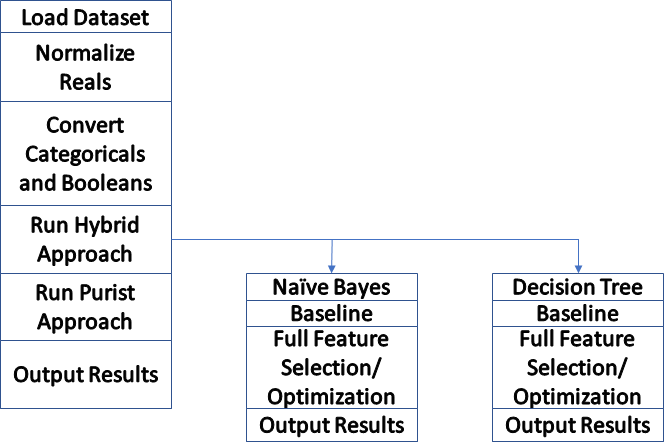
\includegraphics[width=0.7\linewidth]{figures/png/ProgramFlow}
	\caption[Overall Program Flow]{Birds-eye view of the flow of the program. Hybrid approaches are not run in parallel, because at time of coding MATLAB doesn't support multi-threading via a COM server.}
	\label{fig:ProgramFlow}
\end{figure}
Loading and normalization gets all algorithms on the same page, ensuring an apples-to-apples comparison.  First we have the hybrid approaches.  Within a hybrid approach, we first see what optimizing without including features yields- this is referred to in the code and in the program as the hybrid approach.  It has all the same constraints as the parent approach.  After the baseline, we optimize a second time, this time including feature selection, by which we mean that we characterize a dataset with n variables as either included (1) or excluded (0) in a bitstring, and encode the same variables to the classifier as in the baseline method.  We have selected two distinct classifiers: a multiclass na\"ive Bayes algorithm and a simple single decision tree.  Each of these are run twice per dataset- once with feature selection disabled (the baseline) and once with it enabled.  We will discuss those methods in more detail in their respective sections.\\The purist approach is much more straightforward.  There is only one mode which it runs in, there's no explicit feature selection.  That is, there is feature selection, but all features are available to the algorithm at any time- just some may or may not be included. This portion of the algorithm is threaded.  
\section{Preprocessing}
We do some preprocessing of the data.  First and foremost, there is a text file that is read which describes the dataset and points to where it is on the filesystem.  Below is an example- this tells the program where it can find X and Y and how to parse them.\pagebreak
\begin{lstlisting}[language=config]
#Dataset Name
CardioData
#Class Names File
../../../Data/Cardio/classNames.txt
#TrainingSet X Path
../../../Data/Cardio/trainingXY.csv
#TrainingSet Y Path
../../../Data/Cardio/trainingXY.csv
#TestingSet  X Path
../../../Data/Cardio/testingXY.csv
#TestingSet  Y Path
../../../Data/Cardio/testingXY.csv
#X ignore list, comma separated and starting with w if it's a whitelist (otherwise, blacklist)
b, 29, 30
#Y ignore list, as above
w, 29
#Categorical Variables, white/blacklist, comma separated
w, 
#Boolean Variables, as above
w, 
\end{lstlisting}
For instance, in this case X(the data) and Y(the labels) are in the same file, but represented as different columns.  They could easily be stored as two files.  After those files are explained, the next uncommented line describes the columns to ignore or include, specified with b for blacklist or w for whitelist respectively.  In this example, columns 29 and 30 are ignored for X, but only 29 is included for Y.  This is because for this dataset, there are two sets of labels and thus two separate description files to use the file differently.  Using the same notation, we can declare categorical and boolean variables for X.  Y is assumed to be categorical.\\
After we read how to parse the file, we read the files themselves.  At this point we also convert booleans and categorical variables to doubles so that they can fit in the same matrix.  First, however, we want to normalize the Reals.  First we gather max, min and mean from each column in the dataset.  Then we use a function to squeeze the values down between .1 (b) and .9 (t) for reasons that will be seen later in the section on the purist approach.  
$$x_i^{\prime} = b+(b-t)\frac{(x^i-x_i^{min})}{x_i^{max}-x_i^{min}}$$ Next, categorical variables are given the treatment motivated and described fully in \cite{zhang_visual_2015}, the conclusion being that every category label is replaced with a real number which maximizes Pearson's Correlation Coefficient.  That is,
\begin{align*}
X &= {X_\mathbb{R} \cup X_{cat} \cup X_{bool}}\\
X_\mathbb{R} &= \{x_1, x_2, ... x_n\}\\
X_{cat} &= \{x_1, x_2, ... x_c\}\\%there are some number of categorical columns, each of which have a number of categoricals in them.
X_{bool} &= \{x_1, x_2, ... x_b\} \\
1&\leq i \leq c\\
L &= \{x_i|x_i\epsilon X_{cat}\}\\%Set of categoricals
C_l &= \{x, i|  x\epsilon X \wedge x_{n+i} = l\epsilon L \}\\%set of samples belonging to categoricals
\end{align*}
Where X is the dataset, $X_\mathbb{R}$ is the real portion of the dataset, and$ X_{cat}$ and $X_{bool}$ are the categorical and boolean portions.  The index i iterates over the columns of $X_{cat}$, which lets us derive L, which is the set of all categories in the dataset.  L in turn gives us a means of devising $C_l$, that is, the subset of X which consists of all members of x which belong to the category $l$. Now it is possible to look at $C_l$ and determine which values will maximize $r^2$ for each label l, which we here call R(l).
\begin{align}
R(l) &= \frac{\sum_{x\epsilon C_l}\sum_{j=1}^{n}x_j}{|C_l|n}
\end{align} 
It can be seen as the mean of all the other values over $C_l$.  Calculating this in practice is much more straightforward- simply step through X one sample at a time, and maintain running sums and counts for each unique label, calculate the means at the end and then extend $X_\mathbb{R}$ with the newly calculated values.  In the case of multiple categorical columns, unless there is a perfect correlation between two category labels each label will have its own value (though this can't be proven to be unique, only generated from a unique set of numbers).\\
Booleans are only given the treatment of being converted to values .25 for false and .75 for true.  Again, the reasons we don't use 0 and 1.0 will be made clear in the section on our purist approach.\\
Now that the data has been modified, some additional bookkeeping is accomplished.  Conversions to numerics from string class labels and vice versa are computed and stored, since mathematical approaches prefer integers while human-readable outputs are in the terms given us by the dataset.  Also, global values such as Elitism Percentage and Population Size are modified at this point and are effectively constant for the rest of the program.  Variables that may be configured by the user are: Max Generations, Record Interval, Population Size, and Complexity bounds.  The Max Generations sets the stopping condition of the algorithms, and defaults to 100.  The Record Interval determines how often to save data to the disk- data is collected every generation, but is only saved to disk in where $G mod(RI) = 0$, and the default is 25.  Complexity bounds are discussed in more detail in the purist approach, and have no effect on the hybrid approach.  Other modifications to semi-constants are made at this point determining the length of chromosomes for both approaches based on the characteristics of the datasets- particularly the number of features.
\section{Hybrid Approach}
As mentioned previously, the hybrid approach consists of 2 methods which each consist of two different ways of running them.  First we will discuss the multi-class na\"ive Bayes (McNB) approach, followed by the decision tree (DTree) approach.
\paragraph{McNB}
Na\"ive Bayes is one of the most direct of classifiers, but it is powerful and versatile.  Without going into extreme detail, it generates probability distributions for each class across every dimension in the feature set from the training data, and picks the most likely class for a given sample point.  Typically, the probability distributions are Gaussian, however any density function can be used.   We use this because it should provide a fairly low bar to compete with- support vector machines (SVMs) are much more complex, tend to be extremely reliable and robust, and are close to something resembling the industry standard, but don't perform well with multiple classes.  McNB is closer to statistical modeling and is not what we consider machine learning, though no bright line distinction exists.  It is a theoretically grounded but simple statistical method well suited to being a first pass at the data or being used in conjunction with other methods.  Being simple, it is also relatively fast- only 2 passes through the data are necessary to build the parameters for the PDFs, so building the model can be done in linear time.  Once built, checking a given variable can be done in constant time.
\begin{equation}
P(A|B) = \frac{P(B|A)*P(A)}{P(B)}
\end{equation}
The standard formulation of Bayes' theorem, in our case it is more useful to form it thus:
\begin{equation}
P(\omega_j|x) = \frac{p(x|\omega_j)P(\omega_j)}{p(x)}
\end{equation}
Here, $\omega_j$ is the likelihood of belonging to a particular class.  Upper case Ps are simple probabilities, lower case Ps are more complex functions. So $p(x|\omega_j)$ is the PDF, and $P(\omega_j)$ is the prior, which can be thought of as \textit{a priori} how likely a particular class is to present.  To build the PDF, if we're using a Gaussian, we need mean and standard deviation for each class.  The Gaussian PDF is built using the training set, tested on the testing set, and the results are scored in a confusion matrix.  This can be determined from the dataset, in which case it uses the frequency in the Training set to generate priors, or set manually.  In either case, this can be seen to scale a particular PDF.  In fact, this is similar to what p(x) does- except that where $P(\omega_j)$ scales a class, p(x) scales all classes, and it serves as a normalizing constant to constrain values between 0 and 1.  It could be established using the law of total probability, or it could be some arbitrarily high constant.  It doesn't really make a difference, since the selected class will just be the one with the highest score given x, and if it effects all classes equally nothing is served by making complex calculations every time the classifier is called.\\